\chapter{眶额皮层:基于输出结果选择目的}
这本书提出了关于灵长类动物前额叶皮层基本功能的方案。

\section{概述}
眶额皮层有助于评估和选择对象未来行动的目标及其联系解释了其独特的功能。 它与嗅觉、内脏、味觉、体感和皮层的视觉区域,这些信号的结合产生了丰富的,特定结果的高维表示,一个由想象。 眶额皮层与杏仁核更新的相互作用根据当前的生物学需求评估这些成果。由于这些联系,看到有营养的食物或视觉标志与他们相关联唤起他们的味道和他们当前的动机价值。 虽然眶额皮层的很大一部分将物体链接到特定的结果,另一部分对一般结果这样做,在“共同货币”。 通过将行为结果分配给特定的觅食事件,而不是此类事件的平均值,眶额皮层灵长类动物提供了关键的选择优势。
\section{介绍}
第 3 章论证了内侧皮层的连接允许它做出选择在行动中,特别是当这些选择发生在没有外部感官的情况下时告诉动物该做什么的提示。 本章介绍眶额皮层。 它认为眶额皮层的连接允许它为外部提示做选择内侧皮层对“内部”提示的作用。\par
与内侧皮层一样,眶额皮层既有颗粒状部分,也有颗粒状部分。第 2 章论证了早期哺乳动物进化出的颗粒状部分,而颗粒状部分部分在早期灵长类动物中进化。 与第 3 章一样,我们需要利用老鼠的证据深入了解颗粒状的。 原因是一样的:我们对灵长类动物的无颗粒皮层。 也像第 3 章一样,我们需要说什么是粒度部分眶额皮层可以做到其颗粒部分不能做到的。 我们采纳这个想法灵长类动物的眼眶额皮层使用单个事件将特定结果与导致这些结果的选择:一种刺激-结果关联的形式。\par
显然,大多数动物都可以学习刺激-结果关联。巴甫洛夫条件反射依赖于它,就像仪器条件反射依赖于学习行动—结果关联一样。 除了无柄形式,我们假设所有动物物种都可以是仪器和经典条件。 所以我们面临一个挑战:我们需要说什么哺乳动物眶额皮层的颗粒部分以及颗粒部分是什么灵长类动物的眶 额皮层。\par
在本章中,我们区分了刺激-结果关联的两个方面。 首先涉及刺激和结果之间的预测关系:可能性给定刺激就会发生结果。 第二个涉及评估结果在当前生物学需求方面的价值。 这两个方面,我们分别称为关联映射和动机评估,都会影响觅食选择,并且两者需要随着情况的变化而更新。\par
\section{区域}
图 4.1 说明了人类和猴子的眶额皮层,图 2.1 说明了其细分的一个视图。 在猕猴中,第 11 区位于它的喙部,区域 13 和 14 位于更靠后的位置 (Walker 1940)。 在灵长类动物中,大部分皮质具有颗粒状细胞结构,但区域 13 和 14 的尾部是颗粒状的,邻近的前岛叶皮质也是如此。 继 Carmichael 和 Price(1994)之后,我们将所有这些无颗粒区域包括在眶额皮层中。 为了清楚起见,我们有时使用眶额皮层的缩写 OFC。 我们尤其在讨论时这样做OFC的分支机构。\par
我们将区域 12/47 的部分从此处解释的眶额皮层延伸到半球的轨道表面,以及极地皮层(区域 10)。
\begin{figure}[!htb]
	\centering
	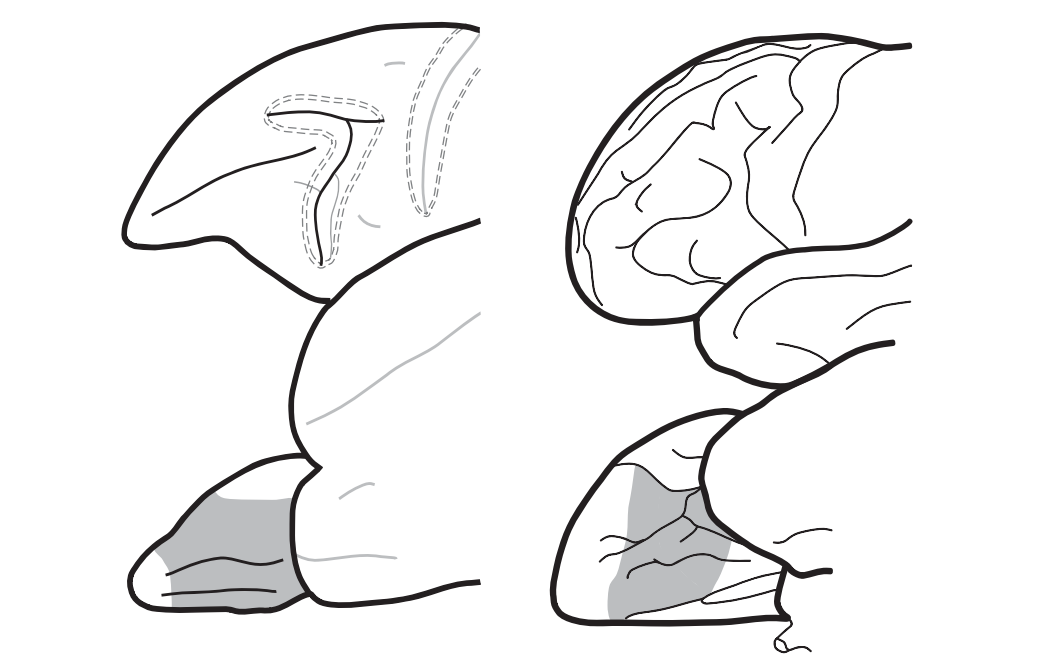
\includegraphics{image_pfc/Fig_4_1}
	\caption{猴子(左)和人类(右)的眶额皮层。 格式如图 1.2 所示。}
\end{figure}


\section{连接}
图 4.2 说明了眶额皮层的选定连接,这表明以下结论:\par
1. 与杏仁核最密集的连接涉及眶额皮层的颗粒部分,优先与杏仁核的基底外侧核连接。然而,13 区的颗粒状部分也与杏仁核有关,其他粒度细分(见图 3.3)(Carmichael \& Price 1995a)。\par
\begin{figure}[!htb]
	\centering
	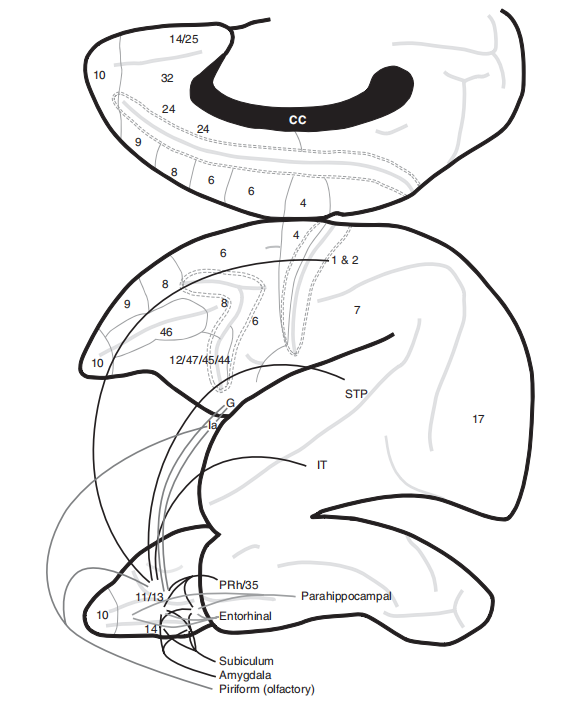
\includegraphics{image_pfc/Fig_4_2}
	\caption{眶额皮层的选定连接。 图 1.4 和 1.5 给出了脑沟和区域的名称。 线连接一些与轨道有直接轴突连接的区域,除非另有说明,否则假设是相连的。}
\end{figure}
2. 无颗粒岛叶皮层接收来自味觉和梨状(嗅觉)皮层(Carmichael \& Price 1995a)。 它还接收来自脑干和丘脑的内脏信号 (Ray \& Price 1992)。 后者包括传达反映动物新陈代谢状态的信号的感觉,例如,缺氧或低血糖,以及来自肺、心脏、压力感受器和消化道 (Craig 2002)。 这些发现导致了这样一种观点,即颗粒状岛叶皮质在内感受中发挥作用。\par
3. 嗅觉、味觉和内脏信息从其到达颗粒状 OFC颗粒部分(Carmichael \& Price 1994)。该信息可以在颗粒皮层中与来自颞下皮层的视觉输入相结合,目标区域 13和 11,以及从投射到区域 13 的鼻周皮质(Saleem 等人,2008 年)。后一种投影提供了关于物体的多模态信息 (Murray et al.
2007 年)。\par
4. S1区和S2区的体感信息也会传到13区,尤其是那些代表喙部(Pritchard et al. 1986)、唇和舌的侧面部分(Carmichael \& Price 1994)。这些联系包括不明确的体感诸如顶叶盖和岛叶颗粒异常部分的区域皮层 (Saleem et al. 2008),以及定义明确的体感区域,例如区域3b 和 S2 本身。 与 S2 的某些联系可能涉及手和口面部表征 (Carmichael \& Price 1994)。\par
5. 与内侧 PF 皮层和腹侧PF皮层(第 3 章和第 7 章)不同,眼眶PF 皮质只有有限的听觉输入 (Saleem et al. 2008)。14区的部分地区其中 13 个与可能提供听觉输入的颞叶区域有联系 (Petrides \& Pandya 1988)。 但是萨利姆等人。(2008) 重新诠释这些连接是根据他们识别的两个连接网络来表示的:轨道和中间网络。他们认为与听觉相关的区域要么是媒体网络的一部分,要么是两个网络的一部分。根据这种观点,眼眶PF皮层的“纯眼眶”部分缺乏听觉输入。原因大概是轨道网络处理有关物体(例如食物)的信息,这些物体具有很少有听觉特征。\par
这些点构成了眼眶 PF 皮层的连接指纹,这表明它是视觉信息与味觉信息汇聚的最早场所,嗅觉和内脏输入。 我们认为大多数视觉输入到达很重要。在灵长类动物特有的颗粒状区域。 因此它不是眼眶 PF 皮层,一般来说,但特别是区域 13 和 11 的颗粒状部分似乎是视觉、嗅觉、味觉和内脏输入之间会聚的最听觉位置。\par
由于这种融合,特定食物的视线,例如特定成熟的阶段的水果,可以唤起它的味道和气味,这构成了它的味道,连同摄入后的内脏感觉。 此外,眼眶 PF 皮层接收来自初级体感皮层的口、唇和舌表征的输入(S1):与食物和液体摄入最相关的身体部位(Carmichael
\& 价格 1995b)。\par
它的连接解剖结构使眼眶 PF 皮层处于一个独特而有趣的位置。 触觉输入提供有关外部环境附近部分的信号; 视觉和嗅觉输入传递来自外部世界遥远部分的信号; 内脏输入告诉动物有关其内部环境的信息; 味觉和口腔体感输入告诉它有关从外部进入内部世界的事物。\par
图 4.3 显示了这些不同的模态和子模态如何组合起来形成联合表征。 其中一些连接发生在无颗粒区域,它们似乎非常适合早期哺乳动物的谷物和昆虫饮食。 这些是专门从事夜间觅食以避免捕食等因素的小动物。 因此,在眼眶 PF 皮层的颗粒部分中表示的连词主要涉及味觉、嗅觉和内脏感觉。 灵长类动物灵长类动物保留了这种基本的特征连接机制,并增加了更大的来自视觉区域的输入。\par
\begin{figure}[!htb]
	\centering
	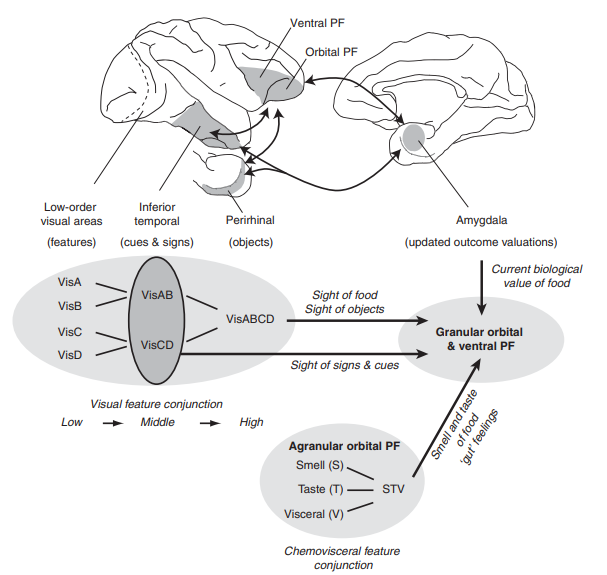
\includegraphics{image_pfc/Fig_4_3}
	\caption{颞叶和额叶皮层的特征连接。 VisA …VisD 指定视觉
		对象的特征,可以组合成各种连接表示,例如 VisAB,
		这表示 VisA 和 VisB 的表示。 “STV”表示物体的气味 (S)、味道 (T) 和内脏 (V) 特性的结合。 转载自 Murray EA, Wise SP,
		Rhodes SE,不同的大脑可以用奖励做什么? 在感觉神经生物学和
		奖励,编辑。 JA Gottfried © 2011,Taylor 和 Francis,经许可。}
\end{figure}

\subsection{概括}
第 3 章认为——通过与海马体、杏仁核和内侧运动前区的联系——内侧 PF 皮层会偏向于在动作之间或在动作之间的选择有关行动的规则。 在那里,我们审查了证据表明它是基于预测结果的当前值这样做的,尤其是当这些选择取决于“内部”信号而不是感官信号时。 本章认为眼眶 PF 皮层执行在外部信号之间进行选择的类似功能,尤其是那些来自物体的信号。 它之所以能够这样做,是因为来自体感、味觉、嗅觉、内脏和视觉皮层以及杏仁核的信息会聚和整合。
\section{啮齿动物的无颗粒皮质}
颗粒状 OFC 在啮齿动物研究中引起了相当大的关注,其中大部分表明在以结果为导向的行为中起着重要作用。 回想一下,在整本书中我们都区分了目标和结果,因此在其他人可能会说目标导向的地方使用术语“以结果为导向”。 OFC细胞的活动反映了结果预测,尤其是关于奖励的特定感官方面的预测(Schoenbaum 等人,1998 年),这些区域的损伤会损害基于以下因素的选择
结果预期,如下一节所述。
\subsection{刺激-结果关联}
正如第 3 章提到的,当前的生物学需求会影响结果的评估。例如,当前对食物或液体的需求越大,a 的值就越大映射到该结果的刺激。 将食物消耗到饱腹感会使该食物贬值,并且还有其他方法可以改变结果的价值。\par
在使用这些替代方法之一降低食物奖励价值的实验中,加拉格尔等。 ( 1999 ) 比较了具有颗粒状 OFC 损伤的大鼠的行为与正常大鼠相比。 首先,他们教老鼠光表示食物供应。当灯亮时,老鼠会靠近灯。 然后加拉格尔等人。 用过的锂氯化物诱发胃肠道疾病,这一过程称为条件性味觉厌恶。稍后进行测试时,在所有疾病痕迹消失后,正常老鼠接近光线比他们生病前更少,或者完全停止接近光线。受伤的老鼠表现不同。 他们比过去更频繁地接近光正常老鼠。 正如第 3 章所解释的,正常大鼠的结果称为贬值影响。 因为受损的老鼠接近了与奖励贬值相关的刺激,可以说,他们在使用刺激-结果关联来判断方面存在缺陷指导行动。\par
皮肯斯等人( 2003 , 2005 ) 使用相同的任务和贬值程序,但对杏仁核和颗粒状 OFC 造成损伤。 两个病变都废除了大鼠的贬值效应。 这些老鼠的行为就好像它们没有从它们身上学到任何东西一样疾病。\par
这些贬值程序的结果类似于第 3 章描述的结果对于内侧 PF 皮层的病变。 内侧 PF 皮层损伤会导致使用结果预测在竞争行为中进行选择时出现障碍。 在许多这样的实验中,没有任何外部提示可以帮助动物做出选择。 颗粒状 OFC 病变,但是,不要破坏这种行动-结果关联(Ostlund \& Balleine 2007)。
相反,它们破坏了使用关于结果的预测来在对象中进行选择。在这些实验中,外部提示会提示选择,从而揭示缺陷学习刺激-结果协会。 这些研究表明,颗粒状 OFC将刺激与结果联系起来,尤其是食物的感官方面,例如它的气味
或味道。\par
伯克等人的一项实验。 ( 2008 ) 支持这一结论。 老鼠首先学会了将一种刺激与一种特定的食物联系起来。 后来他们看到了这种刺激与额外刺激的结合。 当老鼠看到这种复合刺激时,它们得知它与另一种食物有关。 这两种食物有更多或不太一样的适口性和可取性,但它们的味道不同。\par
伯克等人发现大鼠将第二种食物的发生归因于复合刺激的较新部分。 作为这一结论的证据,他们表明他们的老鼠会按下一根杆来产生额外的刺激。 至关重要的是,Burke等人表明如果老鼠在第二次吃饱了就不太可能这样做食物。 因此,老鼠不仅将额外的刺激与第二种食物联系起来,而且使用该关联来评估刺激的当前值。具有颗粒状 OFC 损伤的大鼠未能显示出这些效果。 关系
在复合刺激的较新部分和特定感觉特性之间第二种食物不再影响他们的行为。 这些结果表明颗粒状 OFC 介导刺激和结果之间的映射,尤其是
结果的特定感官方面。\par
稍后,我们强调了粒度 OFC 的重要性和视觉上的进步
灵长类动物。 然而,正如刚才回顾的实验所表明的那样,老鼠也使用视觉
评估结果的刺激,他们的 OFC 从皮质的视觉区域接收到这些刺激。\par
\subsection{费用}
第 3 章解释了动物不仅根据预测的食物或液体做出决定,而且还有获得它们的成本。 例如,与正常大鼠相比,前扣带回晚期皮质受损的大鼠选择越过障碍的次数较少,因此似乎高估努力成本。\par
无颗粒眼眶 PF 皮层的损伤也改变了大鼠估计成本的方式。当在立即的小奖赏和延迟的大奖赏之间做出选择时,正常老鼠在做出选择时会考虑延迟的时间长短。 鲁德贝克等( 2006b ) 报道有眼眶 PF 损伤的大鼠更多地选择小的即时奖励经常比正常老鼠。“冲动”一词已被应用于选择小额奖励很快,并且“耐心”一词已被用于放弃立即奖励以获得一个更大的以后。 所以在 Rudebeck 等人的实验中,眼眶 PF 皮质病变可以据说会诱发冲动。\par
然而,只要稍微改变实验设计,就会得到不同的结果。鲁德贝克等使用了 T 型迷宫,但 Winstanley 等人( 2004 ) 让老鼠在两个杠杆之间进行选择,一个导致单个颗粒,另一个在延迟后导致四个颗粒。 眼眶 PF 病变的大鼠比正常大鼠更频繁地选择延迟奖励的杠杆。有人可能会说他们表现出比正常人更多的“耐心”。 和马里亚诺等人。 ( 2009 ) 让老鼠在 T 迷宫上的黑色或白色目标框之间做出选择,一个框内有小奖励,另一个框内有大量奖励,只有在延迟后才能获得。同样,患有眼眶 PF 病变的大鼠比 Rudebeck 等人研究中的大鼠表现出更多的“耐心”。\par
泽布等人 (2010) 表明,眼眶 PF 病变是否会导致“冲动”或“患者”选择取决于两个因素:一个明确的信号,表明个体大鼠之间的延迟和差异。 他们使眼眶 PF 皮层失活并比较了提示的效果和无意识的延误。 他们的结果表明,对于明显有提示的延迟,失活会增加立即奖励的选择(冲动),而对于无提示的延迟,失活会减少立即奖励的选择(耐心),但仅限于有强烈冲动倾向的老鼠个体。所以我们不能简单地说大鼠眼眶 PF 皮层偏向于冲动或耐心觅食的选择。 但是,它显然以某种方式在评估延迟成本方面发挥了作用以及偏向延迟或立即行动的行为。 正如第 3 章所解释的那样,累加器-跑道模型提供了一种实现这种偏差的简单机制,既可以通过改变产生输出的阈值,也可以通过调制速率
支持进行特定运动的“证据”不断积累. \par
冲动觅食和耐心觅食之间的竞争通常是根据延迟或远距离获得的食物和液体的贬值或折扣来讨论的。 然而,正如斯蒂芬斯等人( 2004 ) 指出,这个术语意味着动物错误地评估了时间和空间上遥远的食物和液体的价值。或者,动物可能会准确评估价值,但会考虑寻找遥远可用资源的固有风险。 \par
Hayden 和 Platt (2007) 建立了一个模型,其中“风险”期权的估值取决于较大收益的预期时间和收益减少的风险。 他们表明,该模型的预测解释了猴子在赌博任务中做出的选择。由于等待更长时间或走得更远所固有的风险,选择开发立即可用的资源并不一定意味着对延迟或更远资源的错误评估。 即使眼前的补丁比别处的“更绿的牧场”价值低,回报更确定。
\subsection{颗粒状岛叶皮质}
基于连接、细胞结构和拓扑结构,眼眶 PF 皮层包括无颗粒岛叶皮层 (Carmichael \& Price 1994)。 如果无颗粒眼眶 PF 皮层将刺激与结果的特定感觉方面相关联,我们可能期望找到邻近的无颗粒岛叶皮层的相关功能。
Balleine 和 Dickinson (2000) 表明,具有包括无颗粒岛叶皮层在内的损伤的大鼠在需要记住特定味道时表现出损伤。 他们在两种情况下对老鼠进行了测试。 在其中一项中,老鼠在两个杠杆之间做出选择,并接受了那种与任一选择相关的食物。 受损的老鼠倾向于避免按下刚刚导致奖励贬值的杠杆。 在第二种情况下,压榨机不再生产任何食物; 也就是说,老鼠在灭绝中进行了测试。 在这种情况下,受伤的老鼠同样地按下了两个杠杆。\par
因为其他实验表明有这些损伤的老鼠可以学习这种消退任务,Balleine 和 Dickenson 得出结论,有损伤的老鼠无法回忆起它们期望通过按下每个杠杆获得的食物的特定感官特性,因此,尽管其中一种食品贬值,但他们同样选择了它们。 尽管他们的病变侵入了位于岛叶皮质皮质尾部的味觉皮质,但这种影响可能是由岛叶皮质皮质病变引起的。\par
Kesner 和 Gilbert (2007) 还测试了老鼠预期奖赏的能力。 老鼠先喝低蔗糖液体,然后喝高蔗糖液体,几天后,它们喝的低蔗糖液体减少了,以便以后消耗更多的高蔗糖液体。 无颗粒岛叶皮层的损伤消除了这种效应。 然而对照试验表明,受损的大鼠仍然可以分辨出两种液体之间的差异。 本实验表明,岛叶皮质受损的大鼠倾向于选择即时奖励,而不是等待更高价值但延迟的奖励。 这结果可能反映出未能预测延迟奖励的属性或冲动的选择。\par
\subsection{概括}
按照本章第 3 章所述,内侧 PF 皮层的颗粒部分似乎使用行动-结果映射和动机评估来偏向行动或有关行动的规则之间的选择。 映射和估值都涉及“内部”信号,两者都可以影响代表特定选择的累加器网络中的活动(第 3 章)。 因此,例如,按下杠杆预测有益结果(例如葡萄干)的“内部”信号以及评估该结果的信号就当前需求而言,两者都为代表压杆行为的累加器网络提供了“证据”。 有了更多这样的“证据”——例如,更强的关联或获得葡萄干的更高动机——网络将更快地达到阈值并“赢得”控制行为的“竞赛”。
相比之下,眼眶 PF 皮层的颗粒部分似乎使用刺激-结果映射以及动机评估来偏向刺激之间的选择。 与行动-结果映射不同,刺激-结果映射依赖于外部的、感官的信号以及内部信号(关于动机),它们也可以影响累加器网络中的活动。
因为这些区域通过它们密集的互连一起工作(Barbas 1988 ;Price \& Drevets 2010),它们允许哺乳动物选择预测最佳结果的行动或刺激,根据当前的动机价值更新。
我们认为,这种能力比缺乏这些皮层区域的祖先物种更具优势(第 2 章)。 由于它们的无颗粒 PF 皮层,哺乳动物可以在面对不断变化的环境时迅速改变觅食选择。 上一章表明,他们可以学习习惯应该盛行或以结果为导向的行为应该盛行的环境,他们可以学习何时应该通过内在或外在规则来引导导航,并且他们可以通过努力来权衡奖励收益 费用。 本章表明他们可以了解“冲动”或“耐心”觅食的背景。
从这个意义上讲,哺乳动物可以获得相互矛盾的行为知识,当环境发生变化时,它们可以用来偏向其他行为控制系统。 第 3 章解释了这如何在神经网络层面发挥作用。 表 4.1 总结了这些与觅食选择相关的想法。 它并不意味着详尽无遗。 例如,我们忽略了巴甫洛夫到工具的转移、差异结果效应和条件强化等现象。 啮齿动物的颗粒状 OFC 损伤会导致这些任务以及本章和表 4.1 强调的任务受损。

\begin{table}[htbp]
	\newcommand{\tabincell}[2]{\begin{tabular}{@{}#1@{}}#2\end{tabular}} %换行指令
	\centering
	\caption{颗粒状 PF 区域对觅食选择的贡献}
	\renewcommand\arraystretch{1.5}	%设置表格内行间距
	\begin{tabular}{llll}
		\toprule 
		区域   &  贡献  \\
		\midrule
		\tabincell{c}{内侧颗粒状PF\\}&根据预测的成本/收益,在多种行动选择中偏向觅食\\&在中等波动环境中偏向于以结果为导向的选择\\&偏向低波动环境的习惯觅食\\&偏向于外在或内在的导航规则\\
		\midrule
		\tabincell{c}{眶额颗粒状PF}&基于结果的预测感官方面的多种刺激之间的偏差觅食\\&偏向于“冲动”觅食以利用可用资源\\&偏向“耐心”觅食以探索遥远的资源 \\ 
		\bottomrule
	\end{tabular}%
\end{table}%

\section{灵长类动物的颗粒区域}
第 2 章和第 3 章讨论了啮齿动物的内侧额叶皮层与灵长类动物的中外侧 PF 皮层(46 区)同源或类似的说法。 没有令人信服的证据支持这一建议,很多人反对。 在这里我们简要地处理一个关于眼眶 PF 皮层的相关争论。\par
\subsection{比较啮齿动物和灵长类动物的颗粒区域}
与灵长类动物的眼眶 PF 皮层不同,大鼠的眼眶PF皮层完全没有颗粒。此外,它具有非常类似于颗粒状但不是颗粒状的连接,部分灵长类眼眶 PF 皮层。 与粒状 PF 皮层不同,它位于 allocortex 附近,并且与粒状 PF 皮层不同,它对自主输出有相对直接的影响。\par
然而,尽管有所有这些证据,一些神经科学家认为大鼠的颗粒状 OFC 对应于猴子的整个 OFC,包括其颗粒区域(Uylings 等人 2003 年;Seamans 等人 2008 年;Schoenbaum 等人2009).第 2 章解释了这个想法采用两种形式之一。 一是老鼠有猴子眼眶 PF 皮层的微型复制品; 另一个是他们融合了所有领域发生在猴子身上。 这两种观点都基于大鼠和猴子眼眶 PF 皮质之间的某些相似性,例如细胞活动、神经化学特性、连接和损伤效应。
但是所引用的相似性并不对应于诊断特征,而诊断特征正是建立同源性所需要的。 正如第 2 章和第 3 章所讨论的,诊断特征将不同的区域区分开来。 以条件反射的消失为例。 尽管有 OFC 损伤的大鼠表现出比正常消退慢(Kolb 等人 1974年),但猴子中仅限于颗粒状OFC的损伤具有相同的效果(Izquierdo 和 Murray 2005 年)(图 4.4),包括颗粒状 OFC 的损伤也是如此 猴子(Butter 1969)。 因此,有问题的相似性——称为眼眶 PF 皮层的区域的病变导致灭绝学习减慢——无助于我们建立同源性。\par
\subsection{细胞活性}
不幸的是,除了我们之前回顾的解剖学知识外,我们对灵长类动物 OFC 的颗粒部分知之甚少。\par
罗尔斯等人 ( 1994 ) 记录了眼眶 PF 皮层中对咸味、苦味、酸味和涩味做出反应的细胞。 从我们对它们记录位置的检查来看,它们似乎主要记录了 13 区和 14 区的颗粒部分,在 13 区的颗粒部分和岛叶皮质的颗粒部分也有额外的细胞群。所有这些区域的细胞都会对口味做出反应。\par
除了味觉输入,视觉和嗅觉输入有助于确定食物和液体的特性。 在 Rolls 和 Baylis 的研究中,眼眶 PF 皮层中的细胞对视觉和味觉的结合以及嗅觉和味觉的结合都有反应。 大多数显示味觉-视觉或嗅觉-视觉连接的细胞发生在眼眶 PF 皮层的尾端。 一些位于岛叶皮质的颗粒状区域,而另一些位于 13 区的颗粒状部分或至少附近。相同的特性发生得更多也位于眼眶 PF 皮层。\par
Rolls 和他的同事还发现,猴子会按下一个杠杆,通过电极刺激第 13 区的颗粒状部分,这表明它们发现这种刺激是有益的(Mora 等人,1980 年)。 刺激 11 区没有这种效果。 所以细胞位于 OFC 更靠后的部分,包括那些对味觉或视觉或气味与味觉的结合有反应的部分,似乎与大脑其他部位的奖赏系统的相互作用比 OFC 的更靠侧部分更直接。\par


\subsection{结论}


